\section{On the Cost of Computation and Using Rational Proofs Multiple Times}

\begin{frame}{Computation Has a Price: Accounting for Costs}
	\begin{columns}
	\column{0.60\textwidth}
	\begin{block}{So far:}
		\textit{Utility(worker)} $ = \function{Reward}$
	\end{block}
	\onslide<2->
	\begin{block}{Now :}
		\textit{Utility(worker)} $= \function{Reward} - \function{Cost}$
	\end{block}
	\column{0.40\textwidth}
	\onslide<3->
	\begin{block}{}
		$R - \tilde{R} \geq \delta \hspace*{\fill} (1) \hspace*{\fill}$
	\end{block}
	\onslide<4->
	\begin{block}{}
		$(R-C) - (\tilde{R}-\tilde{C}) \geq \delta \hspace*{\fill} (2) \hspace*{\fill}$			
	\end{block}
	\end{columns}
	\bigskip
		\onslide<5->
\begin{block}{How to achieve (2) given (1)?}
\end{block}
		\onslide<6->
	\begin{block}{Solution: scale reward appropriately.}
		If (1) holds, then scaling the reward function by a linear function of $C$ is sufficient to obtain (2).
	\end{block}
%[Say we can scale reward appropriately and this works for one-time]
% Say about individual rationality here
\end{frame}

\begin{frame}[t]{We May Still Have Issues with Multiple Proofs}
\large{\textbf{On input $x$:}}
\begin{columns}
	\column{0.5\textwidth}
\begin{block}{Honest prover $P$:}
	\begin{figure}
		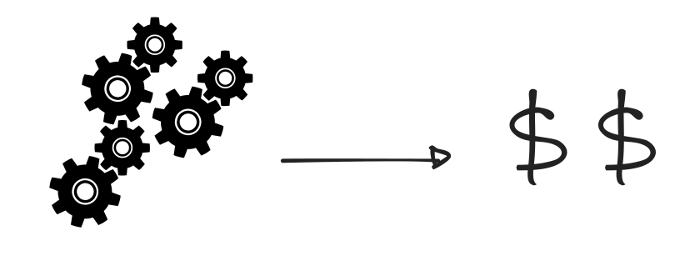
\includegraphics[scale=0.18]{pics/honest-rew.png}
	\end{figure}
\end{block}
\onslide<2->
	\column{0.5\textwidth}
%%%
\bigskip
\begin{block}{Some other prover $\disP$:}
	\begin{figure}
		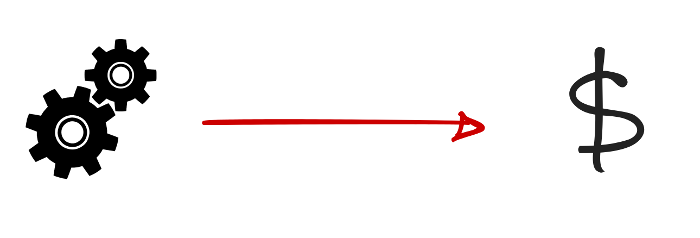
\includegraphics[scale=0.18]{pics/dishonest-rew-one.png}
	\end{figure}
\end{block}
\end{columns}
%%%
\onslide<3->
\large{\textbf{Possible Issue: On multiple inputs $x_1, x_2, x_3$ such prover $\disP$ \underline{profits} more than $P$ on $x$:}}

	\begin{figure}
		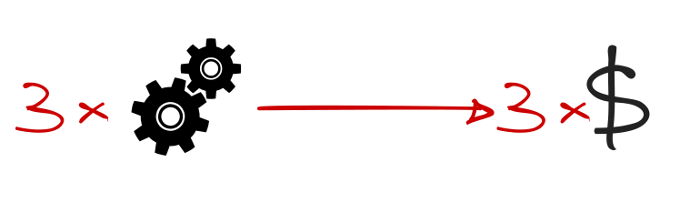
\includegraphics[scale=0.18]{pics/dishonest-rew-many.png}
	\end{figure}

\end{frame}

\begin{frame}[t]{Such Issue Do Occur in Rational Proofs}
	% TODO: Consider scaling between 0 and 1
	% Result: In Micali's protocol for threshold a random strategy is more profitable than an honest one
\large{\textbf{A worker can profit by just replying at random\footnote{A $O(1)$-cost strategy} in protocol by \cite{am1}.}}\onslide<2->
\medskip
\begin{columns}
	\column{0.60\textwidth}
	For a prover giving random answers:
	\onslide<2->
	\begin{align*}
	\tilde{R}_{rnd} > 1
	\end{align*}
	\onslide<3->
	Whereas for the honest prover:
	\[
	R^* \leq 2
	\]\\
	\medskip
	\onslide<4->
Therefore $2\tilde{R}_{rnd} > R^*$
{(It's more profitable to simply cheat twice)}
	\column{0.40\textwidth}
	\onslide<1->
	\begin{figure}
		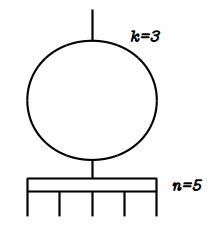
\includegraphics[scale=0.7]{pics/threshold-circ.png}
		
	\end{figure}
\end{columns}
\medskip
	\onslide<5-> \textbf{The protocol in \cite{am1} is not \textit{sequentially composable}}.
	\vfill
\end{frame}

\begin{frame}{Sequential Composability: A Definition}

\begin{framed}
\begin{block}{Desired Guarantee:}
	There should be little gain in doing several, \textit{incorrect} computations instead of a single correct one.
\end{block}
\end{framed}
	\bigskip
\pause
	\begin{block}{Definition}
		A rational proof $(P,V)$ for $f$ 
		is $\epsilon$-{\sf sequentially composable} for an input distribution $\cal D$, if:
			\pause
		\begin{itemize}
			\item  for every prover $\disP$, 
				\pause
			\item	$x,x_1,\ldots,x_k$ drawn according to ${\cal D}$,
		\end{itemize}
				\pause
		$$C(x) \geq \sum_{i=1}^k 
		\tilde{C}(x_i)\implies \sum_{i}\tilde{R}(x_i) - R \leq \epsilon$$
	\end{block}
\end{frame}

\begin{frame}{Sequential Composability: An Alternative Characterization}
\begin{figure}
	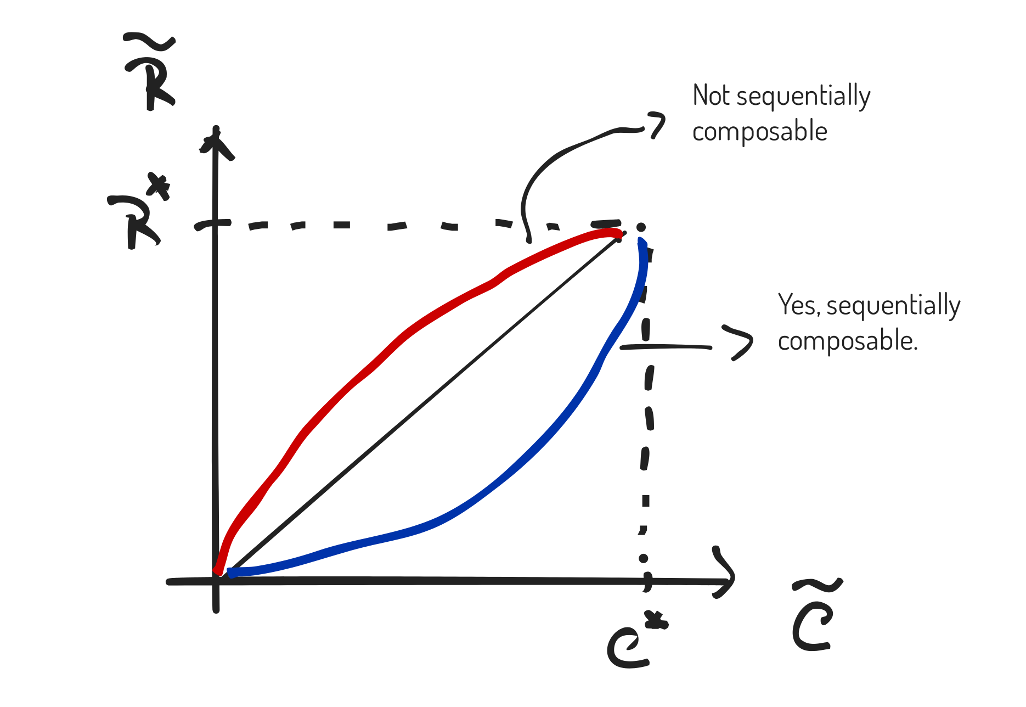
\includegraphics[scale=0.26]{pics/sc-char.png}
\end{figure}
$$ \tilde{C} > \tilde{R}$$
$$ \text{(assuming } R^* = C^* = 1)$$
\end{frame}

\begin{frame}{Space-Bounded Computation and Sequential Composability}
	% Mention cost assumption that we will talk about later
\begin{block}{Theorem (informal)}
	Our Rational Proof for Space Bounded Computation is Sequentially Composable.
\end{block}
\bigskip
\begin{figure}
	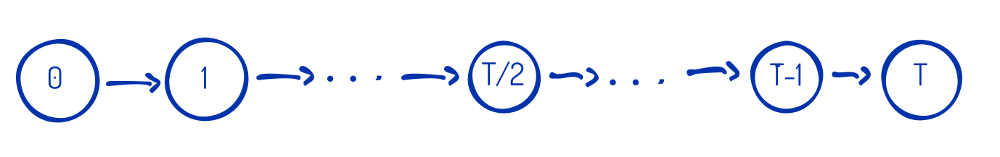
\includegraphics[scale=0.3]{pics/space-protocol.png}
%	\caption{Configuration Graph of a deterministic computation}
\end{figure}
\end{frame}

\begin{frame}[t]{Log-depth Arithmetic Circuits and Sequential Composability}
\begin{block}{Theorem (informal)}
There exist sequentially composable rational proofs for ``regular'' arithmetic circuits of $\log$-depth and $\poly$-size. with:
		\begin{itemize}
			\item $\log n$ rounds;
			\item polylog verifier.
			\item $O(T)$ prover.
		\end{itemize}
\end{block}

\begin{figure}
	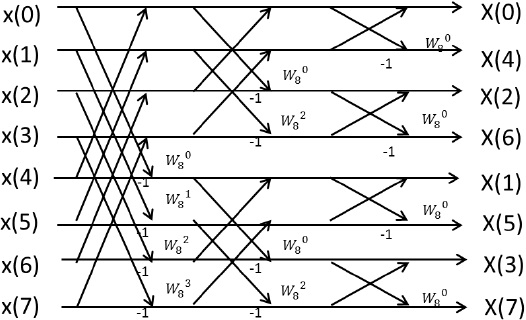
\includegraphics[scale=0.36]{pics/fft.jpg}
	\caption{Circuit for FFT}
\end{figure}
\end{frame}

\begin{frame}{Why Are These Protocols Sequentially Composable?}
	\begin{enumerate}
		\item Reward depends on ``checks'' (although with low soundness);\pause
		\begin{itemize}
			\item Thus, the less the work of the prover the higher the probability of catching him.\pause
			\item Different than earlier approaches where reward depends on \textit{scoring rules}.
		\end{itemize}\pause
		\item Assumptions on costs.
	\end{enumerate}
\end{frame}

\begin{frame}{On Cost Assumptions for Sequential Composability}
\begin{block}{Requirement (connecting cost and probability of guessing)}\pause
{\small 	It should not be too easy to guess a solution having done little work.} 
\end{block}	
	
\pause
\begin{figure}
	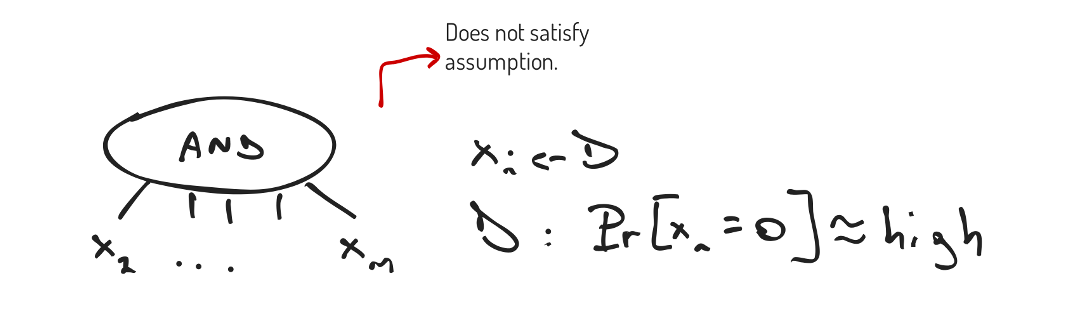
\includegraphics[scale=0.21]{pics/example-and.png}
\end{figure}
\pause
\begin{figure}
	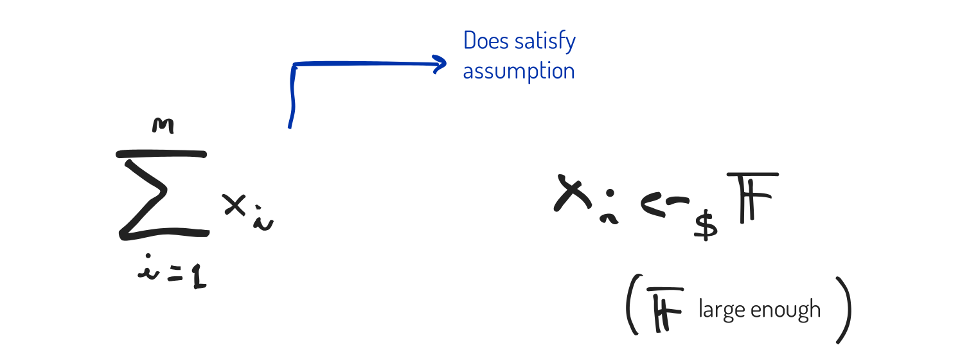
\includegraphics[scale=0.21]{pics/example-sum.png}
\end{figure}
\pause
\textbf{Our assumption:} guessing successfully w/ probability $p$ requires fraction of total work $p$.
\end{frame}